%************************************************
\chapter{Discussion and perspectives}\label{ch:continuity}

In the presented thesis, we have provided the molecular biology background and the biological functions of nucleic acids in general, especially non-coding RNAs. Because of the implication of the secondary structure of non-coding RNAs in performing biological functions, our study focuses on the secondary structure of ncRNAs. Therefore, we have introduced the concepts of RNA bioinformatics and the essential computational problems related to the secondary structure of ncRNAs, such as RNA folding and the inverse problem. We presented a wealthy literature review on existing tools that deal with both problems and some limitations for each tool. Despite very advanced results in the field, we have newly introduced two computation tools: \texttt{RAFFT} and \texttt{aRNAque}. What are the advantages and limitations of those tools? Is there any room for further improvements? How do these tools relate to evolutionary dynamics? In this concluding chapter of our thesis, we will try to provide an answer to these questions by first discussing the advantages and the limitations of the tools previously introduced. 

\section{RAFFT: Limitations and future works }
First, we compared the algorithm performance for the folding task. Two structure estimates were compared with our method: the Thermodynamic-based tools computed using \texttt{RNAfold}, \texttt{LinearFold}, \texttt{RNAstructure} and the ML estimate using \texttt{MxFold2} and \texttt{CONTRAfold}. When we considered the lowest energy structure, the comparison of \texttt{RAFFT} to existing tools confirmed the overall validity of our approach. In more detail, comparison with thermodynamic/ML models yielded the following results. First, the ML predictions performed consistently better than both \texttt{RAFFT} and other approaches, where the PPV $=70.4\%$ and sensitivity $=77.1\%$ on average. Second, the ML methods produced loops, such as long hairpins or external loops. We argue that the density of those loops correlate with the ones in the benchmark dataset, which a PCA analysis revealed too. In contrast, the density of loops was lower in the structure spaces produced by \texttt{RAFFT} and other thermodynamic-based methods, implying some over-fitting in the ML model. Finally, known structures obtained through covariation analysis reflect structures \textit{in vivo} conditions. Therefore, the structures predicted by ML methods may not only result from their sequences alone but also from their molecular environment, e.g. chaperones. We expect the thermodynamic methods to provide a more robust framework for the study of sequence-to-structure relations.
With respect to thermodynamic-based tools, we obtained a substantial gain of performance when analyzing \(N=50\) predicted structures per sequence and not only the lowest energy one. This gain was even more remarkable for sequences with fewer than $200$ nucleotides, reaching the accuracy of ML predictions. 

So how does \texttt{RAFFT} predictions contain structures that are more relevant than the MFE, although these structures are less thermodynamically stable? The interplay of three effects may explain this finding. First, the MFE structure may not be relevant because active structures can be in kinetic traps. Second, \texttt{RAFFT} forms a set of pathways that cover the free energy landscape until they reach local minima, yielding multiple long-lived structures accessible from the unfolded state. Third, the energy function is not perfect, so that the MFE structures computed by minimizing it may not in fact be the most stable. 

We also showed that the fast-folding graph produced by \texttt{RAFFT} can be used to reproduce state-of-the-art kinetics, at least qualitatively. Our method demonstrated three main benefits. First, the kinetics can be drawn from as few as $68$ structures, whereas the barrier tree may require millions. Second, the kinetics ansatz describes the complete folding mechanism starting from the unfolded state. Third, for the length range tested here, the procedure did not require any additional coarse-graining into basins. (Longer RNAs might require such a coarse-graining step, in which structures connected in the fast-folding graph are merged together).

Based on our results, we believe that the proposed method is a robust heuristic for structure prediction and folding dynamics. The folding landscape depicted by \texttt{RAFFT} was designed to follow the kinetic partitioning mechanism, where multiple folding pathways span the folding landscape. This approach has shown good predictive potential. Furthermore, we derived a kinetic ansatz from the fast-folding graph to model the slow part of the folding dynamics. It was shown to approximate the usual kinetics framework qualitatively, although using many fewer structures. 

However, further improvements and extensions of the algorithm may be investigated. For starters, the choice of stems is limited to the largest in each positional lag, a greedy choice which may not be optimal. Furthermore, we have constructed parallel pathways leading to a diversity of accessible structures, but we have not given any thermodynamic-based criterion to identify which are more likely to resemble the native structure. We suggest using an ML-optimized score to this effect. Our method can also find applications in RNA design, where the design procedure could start with the identification of long-lived intermediates and use them as target structures. We also believe that mirror encoding can be helpful in phylogenetic analysis. Indeed, the correlation spectra \(\text{cor}(k)\) computed here contained global information of base-pairing that can be used as a similarity measure.

The versatile method implemented in \texttt{RAFFT} gives possibilities for an alternative application of the FFT in RNA-RNA interaction. The underlying idea is that instead of encoding a sequence $X$ and its mirror sequence $\bar{X}$, one can consider two encoded sequences $X$ and $Y$, and the correlation between them will allow identifying the fraction of high interaction between two RNA sequences quickly. In general, RNA-RNA interaction prediction methods are divided into three groups: alignment like methods, MFE methods and comparative methods. MFE methods constitute the majority of the RNA-RNA interaction tools with the only difference often based on whether the method considers intramolecular interactions, neglects the intramolecular interactions or measures the accessibility of binding region (intra and inter interactions) \cite{umu2017comprehensive, dieterich2013computational, backofen2010computational}. For a preliminary implementation , we neglected intramolecular interactions and intermolecular binding pairs are not allowed to cross. To assess the performance of our naive implementation, we used benchmark dataset also used in the recent review paper on RNA-RNA interactions \cite{umu2017comprehensive}. The dataset consists of   Figure \ref{} shows the  distribution of  different scores: sensitivity, PPV and the MCC compared to other tools scores taken from  \cite{umu2017comprehensive}.

\section{Levy flights and optimisation problems}
The main advantage of using a Lévy flight over local search is a reduction in the number of generations required to reach a target. This is because the infrequent occurrence of a high number of mutations allow a diverse set of sequences among early generations, without the loss of robust local search. One consequence is a rapid increase in the population mean fitness over time and a rapid convergence to the target of the maximally fit sequence. To illustrate that advantage, we ran \texttt{aRNAque} starting from an initial population of unfolded sequences both for a "one point mutation" and "Lévy mutation".

Figures  \ref{Fig:diversity}C and  \ref{Fig:diversity}D show respectively the max/mean fitness over time and the number of distinct structures discovered over time plotted against the number of distinct sequences. When using a Lévy mutation scheme, the mean fitness increases faster in the beginning but stays lower than the one using local mutations. Later in the optimisation, a big jump or high mutation on the RNA sequences produces structures with fewer similarities and, by consequence, worse fitness. In the $(5-10)^{th}$ generation, sequences folding into the target are already present in the Lévy flight population, but only at the $30^{th}$ generation are similar sequences present in the local search population. The Lévy flight also allows exploration of both the structure and sequence spaces, providing a higher diversity of structures for any given set of sequences (Figure \ref{Fig:diversity}D). Using the mean entropy of structures as an alternate measure of diversity, we see in Figure \ref{Fig:diversity}A how a Lévy flight achieves high diversity early in implementation, and maintains a higher diversity over all generations than a local search algorithm. Although the mutation parameters $P_C$ and $P_N$ influence the absolute diversity of the designed sequences, the Lévy flight always tends to achieve a higher relative diversity than local search, all else being equal. 

\begin{figure}[t!]
	\centering
	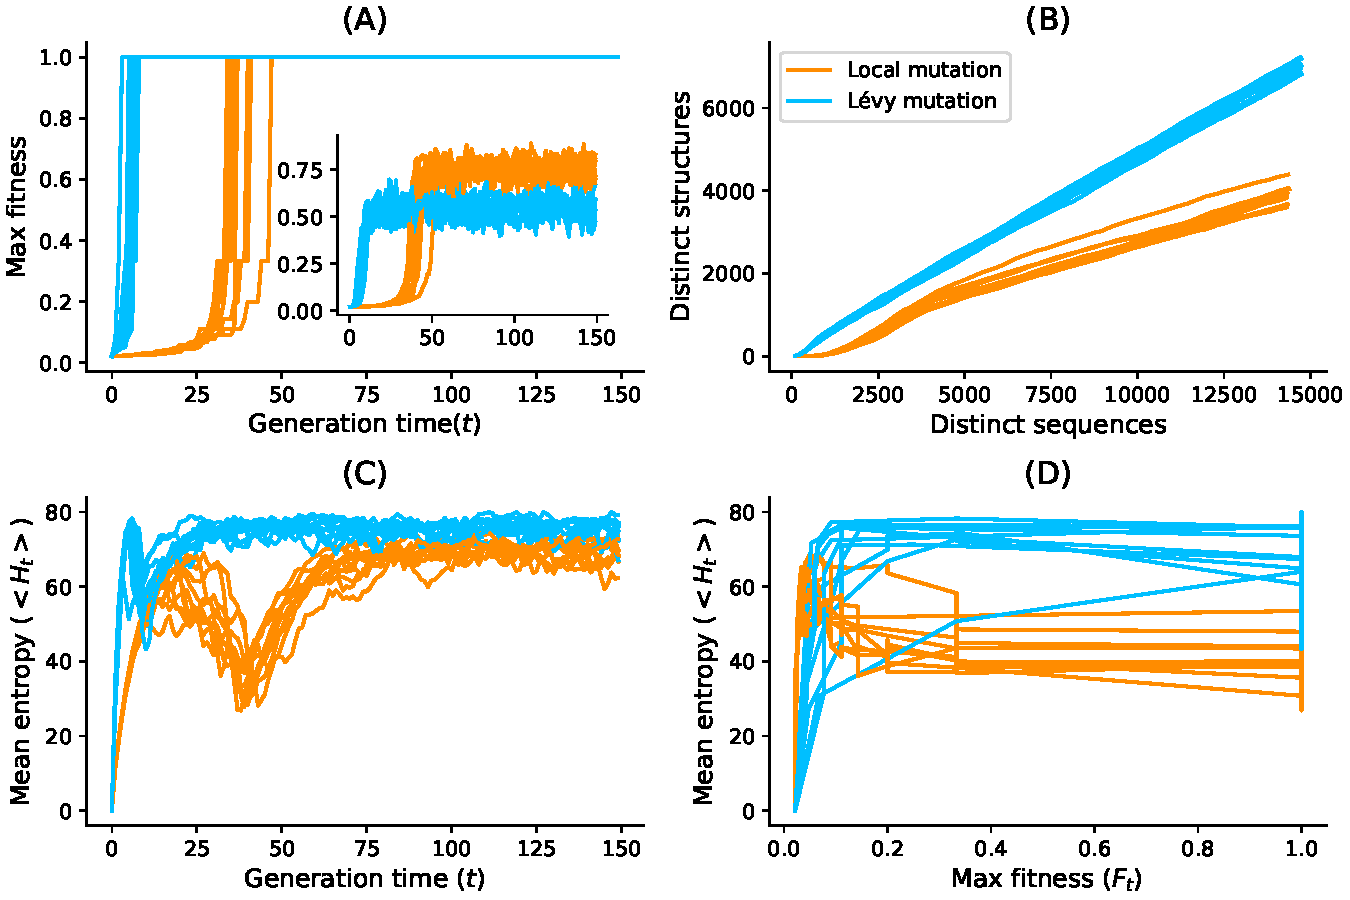
\includegraphics[width=1.0\linewidth]{../res/images/arnaque/fig8.pdf}
	\small 
	\caption{Lévy mutation \emph{vs} one-point mutation: diversity analysis. For the \texttt{Eterna100} target structure \textit{[CloudBeta] 5 Adjacent Stack Multi-Branch Loop}, ten independent runs were performed in which a minimum of $10$ sequences were designed per run.  (A) Max fitness and mean fitness (inset) over time. (B) Distinct sequences \emph{vs.} Distinct structures over time. (C) Mean Shannon entropy of the population sequences over time for both binomial and Lévy mutation. (D) The max fitness plotted against the entropy over time.}
	\label{Fig:diversity}
	
\end{figure}

We argue that the improved performance of the Lévy Flight over local search in target RNA structures is due to the high base pair density of pseudoknotted structures. Given that pseudoknots present a high density of interactions, there are dramatic increases in possible incorrect folds and thus becoming trapped near local optima \cite{hajdin2013accurate}. Large numbers of mutations in paired positions, as implied by a heavy tailed distribution, are necessary to explore radically different solutions. 

To illustrate that Lévy Flight performance was due to base pair density, we clustered the benchmark datasets into two classes: one cluster for target structures with low base pair density (density $\leq 0.5$) and a second cluster for structures with high base pair density (density $> 0.5$). Figure \ref{Fig:diversity2}B shows the number of target sequences available in each low and high density category. The number of targets available in each category are colored according to the percentage of pseudoknot-free targets (\texttt{Eterna100-V1}) vs. targets with pseudoknots (\texttt{Pseudobase++}), showing that pseudoknots are strongly associated with high base pair densities: $71\%$ of the pseudoknotted target structures have a high base pair density.  In contrast, the \texttt{Eterna100} dataset without psuedoknots has somewhat higher representation at low base pair density. If it is true that improved Lévy Flight performance is indeed tied to base pair density, it is possible that similar heavy-tailed mutation schemes could offer a scalable solution to even more complex inverse folding problems. 
\begin{figure}[t!]
	\centering
	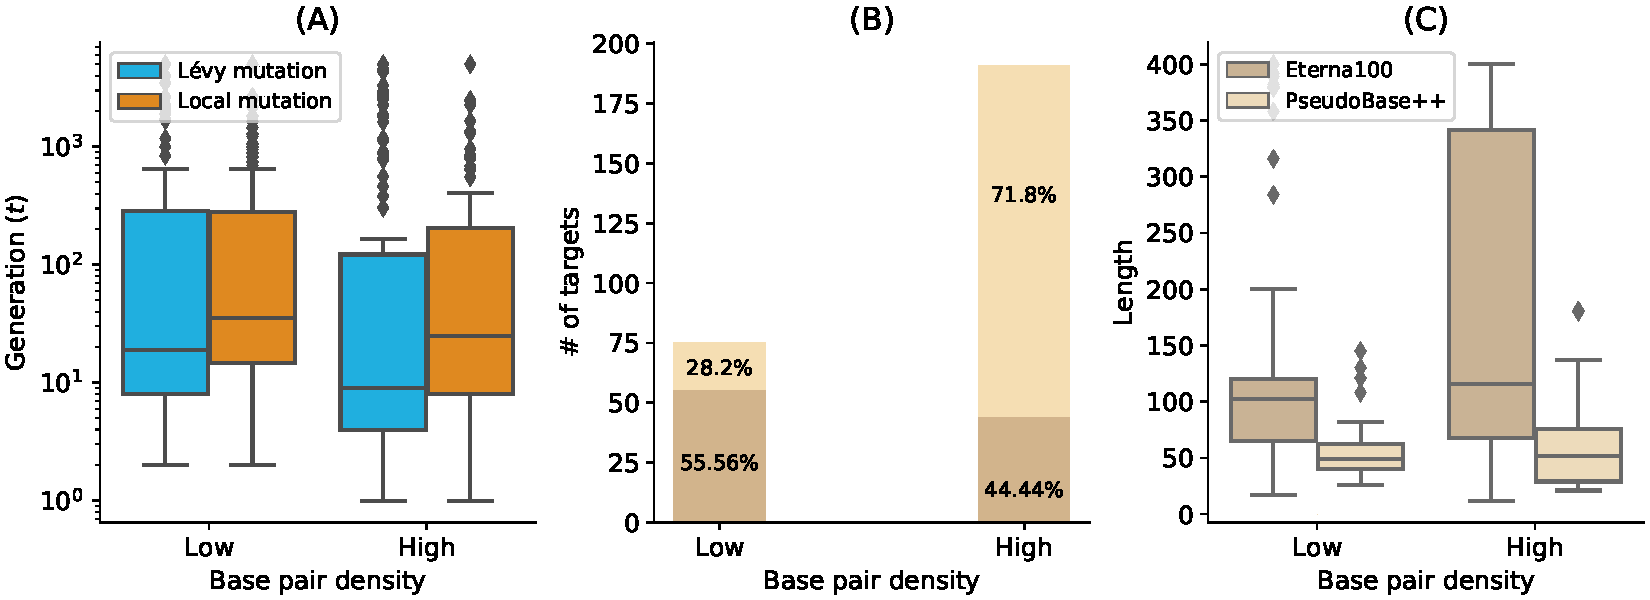
\includegraphics[width=1.05\linewidth]{../res/images/arnaque/fig10.pdf}
	\small
	\caption{Lévy mutation \emph{vs.} Local mutation: performance analysis with respect to the base-pair density. The higher the base-pair density is, the more useful the Lévy mutation scheme to speed up the optimization EA. (A) Distributions of number of generations for the low and high base-pair density targets of the \texttt{Eterna100} dataset. (B) Percentages of targets with low and high base-pair density for the \texttt{Eterna100} and \texttt{PseudBase++}. (C) The length distributions of the low and high base-pair density pseudoknot-free and pseudoknotted targets.} \label{Fig:diversity2}
\end{figure}

A further effort have been made to understand the cases in which the Levy flight mutation can outperform the Binomial with low mutation rate or a constant one-point mutation rate.
The key point of a Levy for the Inverse folding problem partially may rely on the base-pair density and the stability of stems with budge.  

To further illustrate that advantage, we considered the space of all RNA sequences of length  $12$ and with only G,C nucleotides. The structures with the lowest neutral set are: 

\begin{enumerate}
	\item $T_1= ((((...)).))$ : only $2$ sequences fold into the secondary structure $T_1$
		\item $T_2= ((.((...))))$ : only $1$ sequence folds into the secondary structure $T_2$
\end{enumerate}

When having a close look at those two structures the base pair density is maximal and there is an unpaired position on both that allows the formation of a budge. 

What that means naively is that any compatible sequence to $T_1$ (or $T_2$) will likely fold into a stem with four or three base pairs( $((((...)))).$ Or $(((....)))..$ ) , and these particular structures have respectively $243$ and $249$ sequences in their neutral sets. 

We claim that, when having such kind of structure ($T_1$ or $T_2$), the levy mutation is of an important role to get out of the huge neutral network of more stable stems. A simple test case was to run \texttt{aRNAque} for a target secondary structure $T_1$.  For both one point and Lévy mutations, the distribution of the number of generations needed to find sequences that fold into $T_1$ for both mutation schemes is plotted in Figure \ref{fig:target1}. 

\begin{figure}[H]
	
\includegraphics[width=1.0\linewidth]{../res/images/aRNAque/Target1.pdf}
	\caption{Distribution of number of generations need to solve the target $T_1$, for both Lévy and Local mutation schemes. }
	\label{fig:target1}
\end{figure}
Although we believe that Lévy flight-type search algorithms offer a valuable alternative to local search, we emphasise that its enhanced performance over say \texttt{antaRNA} is partially influenced by the specific capabilities of existing folding tools. Their limitations may account for the degradation of these tools as the pseudoknot motifs get increasingly complex. Another possible limitation is that most pseudoknotted and pseudoknot-free target structures are relatively easy to solve (in less than $100$ generation time), requiring more investigations for the unsolved targets to illustrate the performance of the Lévy mutation better.


\section{RAFFT and evolutionary dynamics perspectives}
The RNA inverse folding has deep connections with theoretical evolutionary dynamics studies, where the sequence-secondary structure relationship is a popular model for studying the genotype/phenotype maps [9,20 Yannreview].  Similar to the algorithm implemented in \texttt{aRNAque}, simulating an evolutionary dynamic process using RNA sequence-secondary structure relationship as model often consists of involving a population of RNA sequences to a given target secondary structure. In such simulation, three main ingredients are required: the replication, selection and mutation. These are the fundamental and defining principles of biological systems. The underlying idea is that the genomic material (which is the blueprint that determines the corresponding secondary structure) in form of RNAs is replicated and passed on to the new offspring from generations to generations. At each generation, an RNA individual is then folded into its corresponding secondary structure. A fitness is then defined as a function that measure how close is the realised structure to the target structure. Therefore, selection results when different type of RNA individuals complete with each other. One RNA may reproduce faster and thereby out complete the others. Occasionally, reproduction involves mistakes, these mistakes are termed mutations. Mutations are then responsible of generating different RNAs that can be evaluated in the selection process, thus results in biological novelty and diversity. 

Such a simple genotype/phenotype model gives an unified framework in which concepts in evolutionary dynamics such as: plasticity, evolvability, epistasis, neutrality, continuity and modularity can be precisely defined and statistically measured. At the molecular level, the plasticity is viewed as the capacity of an RNA sequence to assume a variety of energetically favourable secondary structure by equilibrating among them at a constant temperature [Fontana and Laurent W.]. Such concept have been studied in more details using the RNA inverse folding as a toy model. These studies revealed that selection leads to the reduction of plasticity and therefore, to extreme modularity. Another well studied property of evolution is the neutrality which was first introduced by Kimura [the theory of neutral evolution and it suggested that the majority of genotypic changes (or mutations) in evolution is selectively neutral. The attention on Kimura's contention has led to the discovery of neutral network in the context of  genotype-phenotype  models  for  RNA  secondary  structure [4-5]. Two RNA sequences are neutral if they have the same fitness and therefore, they fold into the same RNA secondary structure. The neutrality  is  a central concept in the study of neutral evolution and many recent studies use the sequence-secondary structure relationship as a toy evolution model. 

\begin{figure}[t!]
	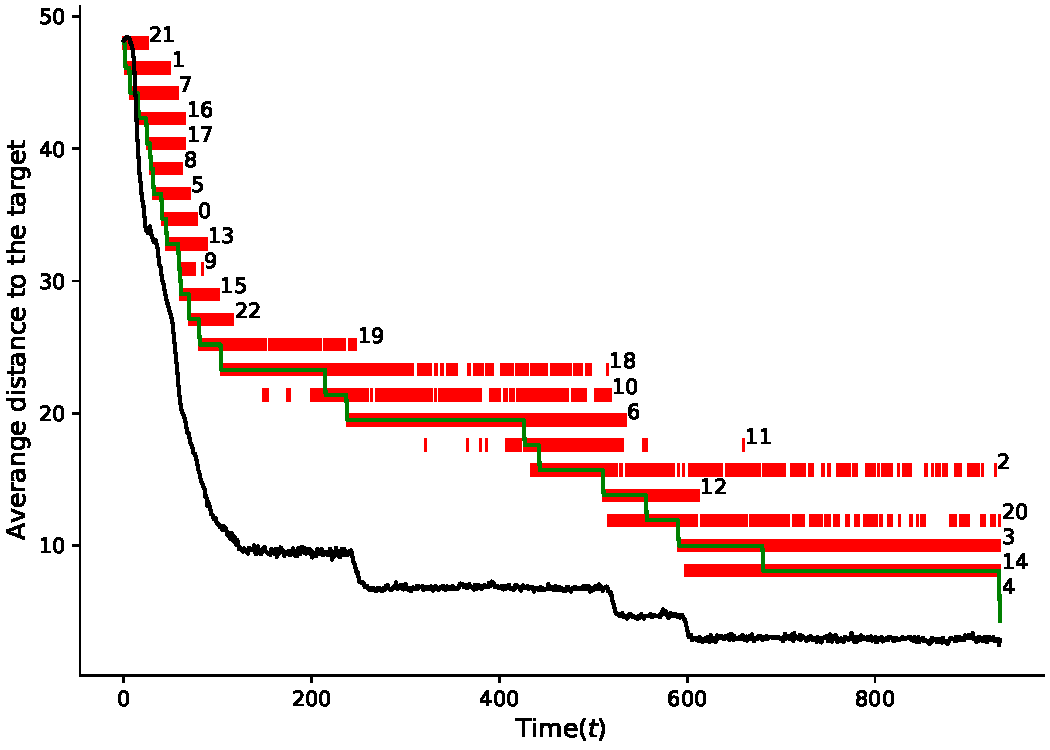
\includegraphics[width=1.0\linewidth]{../res/images/continuity_RNAfold.pdf}
	\caption{Simulation of the an RNA population evolving toward a tRNA (See the figure on the right side) target secondary structure. The target was reached after $933$ generations (i.e. $\approx 10^5$ replications). The black line shows the average structure distance of the structures in the population to the target structure.  The evolutionary history linking the initial structure to the target structure comprises $23$ structures. Each of those structure is labelled by an integer taken from $0$ to $22$. To each of them corresponds one horizontal line (in red). The top level corresponds to the initial structure and the bottom the target structure. At each level, a series of red intervals corresponds to the time periods when the structure was present in the population and the green curve represents the transition between structures. For the red and green curves, only the time axis has a meaning. }
	\label{fig:contiuity}
\end{figure}
Another important issue in evolutionary biology concerns the extent to which the history of life has proceeded gradually or has been punctuated by discontinuous transitions at the level of phenotypes. To distinguish the notion of continuous from discontinuous changes at the level of phenotypes, a notion of nearness between phenotypes has been introduced by Fontana and Peter [45]. The nearness between two structures is based on the probability of one phenotype being accessible from another through changes in the genotype.  Using the RNA sequence-secondary structure relationship makes the notion of discontinuity transition more precise and to understand how it arises in the model of evolutionary adaptation. This is done by simulating an RNA population that evolve toward a tRNA target secondary structure in a flow reactor logistically constrained to a capacity of $1000$ sequences. Once the target secondary structure is found, the evolutionary trajectory is backed to identify all the distinct structures involved and the transition between then. Figure \ref{fig:contiuity} shows the evolution of the average distance to the tRNA target structure, the intervals of time for which a particular structure is present in the population and a transition between distinct structures presents in the evolutionary path. In Fontana's suggestions, a transition ($S_1 \rightarrow S_2$) between two structures $S_1$ and $S_2$ is considered to be continuous if the structure $S_1$ is 'near' $S_2$. In other terms $S_2$ is likely to be accessible through the neighbour neutral sequences of $S_1$. So if $S_2$ appears in the evolutionary path at time $t$, there exists a time $t'<t$ where $S_2$ was already present in the population. In contrast, the transition is discontinuous otherwise (i.e. the time the structure $S_2$ appears in the evolutionary path exactly at the same time it was present in the population).  An example of continuous transition in Figure \ref{fig:contiuity} is the transition  $18 \rightarrow 10$ whereas the transition $15 \rightarrow 22$ is said to be discontinuous. 

\graffito{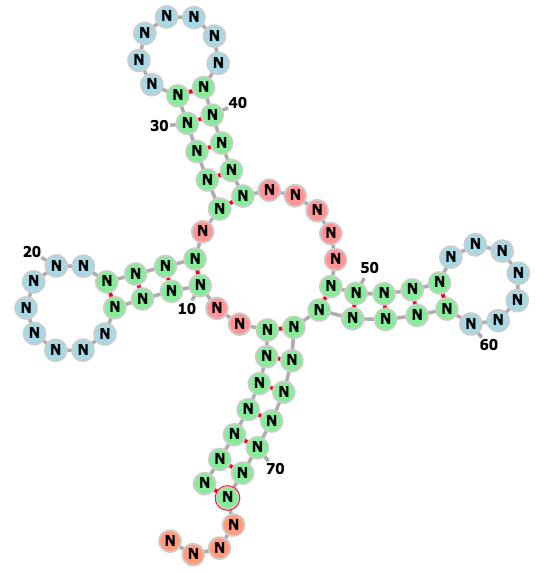
\includegraphics[width=1\linewidth]{../res/images/tRNA_target.png}
	tRNA target secondary structure..}

The previous simulation was performed using \texttt{RNAfold}, the folding tool included in the\texttt{ViennaRNA} package. When using ViennaRNA, the plastic ensemble of an RNA sequence $\phi$ is often considered to be the suboptimal ensemble structure $\Sigma_{\phi}$ within a user-defined energy range above the MFE  at a constant temperature $T$. The \texttt{ViennaRNA} package provides an efficient tools \texttt{RNAsubopt} allowing to compute $\Sigma_{\phi}$.  In a more rigorous implementation of plasticity, each of those structures in the ensemble $\Sigma_{\phi}$ should result from a developmental pathway. Therefore, the environmental changes may induce a change in the developmental path, allowing switching from one structure in the structural ensemble to another. When considering the set of structures produced using \texttt{RAFFT}, each meta-stable structure represents an RNA pathway; this ensemble can therefore be considered as a developmental plastic ensemble. Using RAFFT to simulate the evolutionary dynamic model may provide an alternative framework to study evolutionary concepts like continuity and plasticity. Perhaps, another way of defining continuous transition ($S_1\rightarrow S_2$) from structure $S_1$ to $S_2$ when using will be to check if the structure $S_2$ is in the \texttt{RAFFT}'s structure ensemble of the sequence with MFE $S_1$. In that wise, we suggest utilizing \texttt{RAFFT} to study and draw a different interpretation of continuous evolutionary transition.


